\documentclass[11pt,a4paper]{article}

\usepackage[T1]{fontenc}
\usepackage[margin=1in]{geometry}
\usepackage{amsmath}
\usepackage{amssymb}
\usepackage{array}
\usepackage{booktabs}
\usepackage{xcolor}
\usepackage{tikz}
\usetikzlibrary{arrows.meta,positioning,calc,shapes.gates.logic.US}

\title{ELEC5803 HLS Exam Study\\Step-by-Step Solution to Question 4}
\author{}
\date{}

\tikzset{
  >={Latex[length=2mm]},
  dot/.style={circle, fill, inner sep=1.4pt},
}

\begin{document}
\maketitle

\section*{Course-slide basis}
This solution follows the \textbf{sensitive path algorithm}, \textbf{fault coverage}, and \textbf{test coverage} definitions from
\texttt{Slides/ELEC5803\_Slides10\_Testability and Dependability\_AA2.pdf}.

\section*{1. Interpreting the circuit}
From the gate symbols in the exam figure, the labeled nodes are interpreted as
\[
\begin{aligned}
D &= A\cdot B,\\
E &= B + C,\\
F &= B\cdot C,\\
H &= E\cdot F,\\
G &= D + H.
\end{aligned}
\]

So the circuit can be redrawn as:

\begin{figure}[h!]
\centering
\resizebox{0.9\textwidth}{!}{%
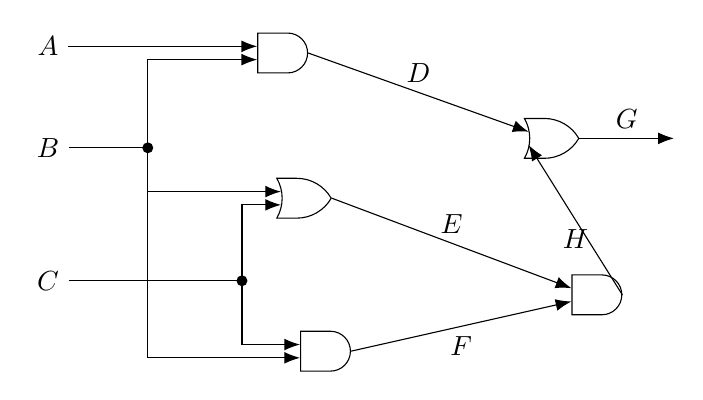
\begin{tikzpicture}[node distance=10mm and 12mm]
  \node (A) {$A$};
  \node[below=8mm of A] (B) {$B$};
  \node[below=12mm of B] (C) {$C$};

  \node[and gate US, draw, logic gate inputs=nn, right=24mm of A, anchor=input 1] (g1) {};
  \node[or gate US, draw, logic gate inputs=nn, below=15mm of g1, anchor=input 1] (g2) {};
  \node[and gate US, draw, logic gate inputs=nn, below=16mm of g2, anchor=input 1] (g3) {};
  \node[and gate US, draw, logic gate inputs=nn, right=28mm of g3, yshift=8mm, anchor=input 1] (g4) {};
  \node[or gate US, draw, logic gate inputs=nn, right=28mm of g1, yshift=-10mm, anchor=input 1] (g5) {};

  \draw[->] (A) -- (g1.input 1);
  \draw[->] (B.east) -- ++(10mm,0) coordinate (bmain) |- (g1.input 2);
  \draw[->] (bmain) |- (g2.input 1);
  \draw[->] (bmain) |- (g3.input 2);

  \draw[->] (C.east) -- ++(22mm,0) coordinate (cmain) |- (g2.input 2);
  \draw[->] (cmain) |- (g3.input 1);

  \draw[->] (g1.output) -- node[above] {$D$} (g5.input 1);
  \draw[->] (g2.output) -- node[above] {$E$} (g4.input 1);
  \draw[->] (g3.output) -- node[below] {$F$} (g4.input 2);
  \draw[->] (g4.output) -- node[below] {$H$} (g5.input 2);
  \draw[->] (g5.output) -- node[above] {$G$} ++(12mm,0);

  \node[dot] at (bmain) {};
  \node[dot] at (cmain) {};
\end{tikzpicture}%
}
\caption{Native-LaTeX redraw of the Q4 circuit.}
\end{figure}

\section*{2. Stuck-at fault list}
The question asks about points $(A,B,C,D,E,F,G,H)$. Under the single stuck-at fault model, each point may be stuck at 0 or stuck at 1.

Therefore the full fault list has
\[
8 \times 2 = 16
\]
faults:
\[
\{A/0,A/1,B/0,B/1,C/0,C/1,D/0,D/1,E/0,E/1,F/0,F/1,G/0,G/1,H/0,H/1\}.
\]

\section*{3. Part (a): minimum test pattern set using the sensitive path algorithm}
\subsection*{3.1 Sensitive path method from the slides}
The slides summarize the method as:
\begin{enumerate}
  \item select a fault,
  \item force the faulty node to the opposite logic value in the fault-free circuit,
  \item sensitize a path from that node to an observable output,
  \item check consistency,
  \item use one test to cover as many faults as possible.
\end{enumerate}

\subsection*{3.2 Derive representative tests}
\paragraph{Test 1: detect $A/0$}
To detect $A/0$, the fault-free value at $A$ must be 1, so set
\[
A=1.
\]
Since $A$ is only observable through
\[
A \rightarrow D \rightarrow G,
\]
we must make
\[
B=1
\]
so that $D=A\cdot B$ depends on $A$.

Also, the other OR input must be 0 so that $D$ is visible at $G$:
\[
H=0.
\]
One simple choice is
\[
C=0 \Rightarrow F=B\cdot C=0 \Rightarrow H=E\cdot F=0.
\]
Hence a valid test is
\[
\boxed{110/10}
\]
where the fault-free output is $(G,H)=(1,0)$.

\paragraph{Test 2: detect $A/1$}
To detect $A/1$, force the fault-free value
\[
A=0.
\]
Again choose
\[
B=1
\]
to let $D$ depend on $A$, and choose
\[
C=0
\]
to force $H=0$ and sensitize the path to $G$.

So another valid test is
\[
\boxed{010/00}.
\]

\paragraph{Test 3: detect $E/0$}
To detect $E/0$, the fault-free value at $E$ must be 1:
\[
E=B+C=1.
\]
To observe $E$ through
\[
E \rightarrow H \rightarrow (H,G),
\]
the other input of the AND gate must be 1:
\[
F=1.
\]
Since
\[
F=B\cdot C,
\]
this requires
\[
B=1,\quad C=1.
\]
Using
\[
A=0
\]
avoids unnecessary masking through $D$.

Thus a valid test is
\[
\boxed{011/11}.
\]

\paragraph{Test 4: detect $B/1$}
To detect $B/1$, the fault-free value at $B$ must be 0:
\[
B=0.
\]
Choose
\[
A=0,\quad C=1.
\]
Then in the fault-free circuit:
\[
D=0,\quad E=1,\quad F=0,\quad H=0,\quad G=0.
\]
If $B$ is stuck at 1:
\[
E=1,\quad F=1,\quad H=1,\quad G=1.
\]
So the fault is observable at both outputs.

Hence a valid test is
\[
\boxed{001/00}.
\]

\subsection*{3.3 Minimum test set}
Collecting the four tests above:
\[
\boxed{
T=\{001/00,\;010/00,\;011/11,\;110/10\}.
}
\]

This set detects all detectable faults of the circuit.

\subsection*{3.4 Faults covered by each test}
\begin{center}
\begin{tabular}{ll}
\toprule
Test vector & Faults detected \\
\midrule
$001/00$ & $B/1,\; D/1,\; F/1,\; G/1,\; H/1$ \\
$010/00$ & $A/1,\; C/1,\; D/1,\; F/1,\; G/1,\; H/1$ \\
$011/11$ & $B/0,\; C/0,\; E/0,\; F/0,\; G/0,\; H/0$ \\
$110/10$ & $A/0,\; B/0,\; C/1,\; D/0,\; F/1,\; G/0,\; H/1$ \\
\bottomrule
\end{tabular}
\end{center}

\subsection*{3.5 Untestable fault}
The only undetectable fault is
\[
\boxed{E/1}.
\]

\paragraph{Reason:}
To detect $E/1$, the fault-free circuit must have
\[
E=0.
\]
But to propagate $E$ through the AND gate to $H$, we must also have
\[
F=1.
\]
Since
\[
F=B\cdot C,
\]
$F=1$ implies
\[
B=1,\quad C=1.
\]
However then
\[
E=B+C=1,
\]
which contradicts the requirement that the fault-free value of $E$ be 0.

Therefore no sensitive path test exists for $E/1$.

\section*{4. Part (b): fault coverage and test coverage}
From the slides:
\[
FC=\frac{N_{\text{det}}}{N}\times 100\%,\qquad
TC=\frac{N_{\text{det}}}{\hat{N}}\times 100\%
\]
where:
\begin{itemize}
  \item $N$ = total number of faults,
  \item $N_{\text{det}}$ = number of detected faults,
  \item $\hat{N}$ = number of detectable faults.
\end{itemize}

\subsection*{4.1 Count the faults}
\[
N=16.
\]
Since only $E/1$ is undetectable,
\[
\hat{N}=15.
\]
Our test set detects all detectable faults, so
\[
N_{\text{det}}=15.
\]

\subsection*{4.2 Fault coverage}
\[
FC=\frac{15}{16}\times 100\%=93.75\%.
\]

\subsection*{4.3 Test coverage}
\[
TC=\frac{15}{15}\times 100\%=100\%.
\]

\subsection*{4.4 Final answer for part (b)}
\[
\boxed{FC=93.75\%,\qquad TC=100\%.}
\]

\section*{5. Part (c): observability and testability of each point}
\begin{center}
\begin{tabular}{>{\raggedright\arraybackslash}p{1cm} >{\raggedright\arraybackslash}p{3cm} >{\raggedright\arraybackslash}p{7.2cm}}
\toprule
Point & Observability / testability & Discussion \\
\midrule
$A$ & Good controllability, medium observability & As a primary input, $A$ is easy to set to 0 or 1. It is observable only through $D$ and then $G$, so the path must be sensitized by forcing $B=1$ and $H=0$. Both $A/0$ and $A/1$ are detectable. \\
$B$ & Good controllability, good observability & $B$ fans out to $D$, $E$, and $F$, so changes at $B$ can affect both $H$ and $G$. This gives several detection opportunities, and both stuck-at faults are detectable. \\
$C$ & Good controllability, medium observability & $C$ affects $E$ and $F$, then reaches outputs through $H$ and $G$. It is less directly observable than $B$, but both $C/0$ and $C/1$ are still detectable. \\
$D$ & Good observability when $H=0$ & $D$ reaches the output only through the final OR gate, so to observe $D$ we must force the other OR input to 0. Hence $D$ is reasonably testable, but only after sensitization. \\
$E$ & Poor observability, poorest testability & $E$ is observable only through $H=E\cdot F$, so we need $F=1$ to make $E$ visible. This allows testing $E/0$, but makes $E/1$ impossible to test. Thus $E$ is the weakest point in the circuit. \\
$F$ & Good observability when $E=1$ & $F$ can be observed at $H$ and then at $G$, provided the other AND input is set to 1. Both stuck-at faults are detectable. \\
$G$ & Highest observability & $G$ is a primary output, so any fault effect reaching $G$ is directly visible. Both $G/0$ and $G/1$ are easy to test. \\
$H$ & Very high observability & $H$ is directly labeled as an observable node and also feeds $G$. This makes it one of the easiest internal nodes to observe and test. \\
\bottomrule
\end{tabular}
\end{center}

\section*{6. Final exam-style answers}
\subsection*{(a)}
Using the sensitive path algorithm, a minimum test set is
\[
\boxed{T=\{001/00,\;010/00,\;011/11,\;110/10\}.}
\]

\subsection*{(b)}
The set detects 15 of the 16 stuck-at faults. Since only $E/1$ is undetectable:
\[
\boxed{FC=93.75\%,\qquad TC=100\%.}
\]

\subsection*{(c)}
Among all points, $E$ has the poorest observability and testability because one of its stuck-at faults ($E/1$) is untestable. Points $G$ and $H$ have the best observability because they are directly observable outputs / output-near nodes.

\end{document}
